%----------------------------------------
% Preamble to set up the document
%----------------------------------------
\documentclass{article}

% set up packages (you shouldn't need to touch this)
\usepackage{graphicx}  % required to insert images
\usepackage{hyperref}  % for hyperlinks
\usepackage[svgnames]{xcolor}  % to change hyperlink colors
\colorlet{linkcolour}{DarkBlue}
\hypersetup{colorlinks=true, linkcolor=linkcolour, citecolor=linkcolour, urlcolor=linkcolour,}

% Margins
\topmargin=-0.45in
\evensidemargin=0in
\oddsidemargin=0in
\textwidth=6.5in
\textheight=9.0in
\headsep=0.25in

% use a sans serif font
\renewcommand{\familydefault}{\sfdefault}

%----------------------------------------
% Step 1: Edit the lecture title
%----------------------------------------
\title{
Lecture 6: Reproducibility, replication, etc., Part 2 \\  % Lecture title
Modeling Social Data, Spring 2018 \\   % Course title
Columbia University                    % School
}

%----------------------------------------
% Step 2: Edit your name and the date
%----------------------------------------
\author{Sang Won Lee}                     % Scribe's name
\date{March 01, 2019}                % Lecture date

\begin{document}

\maketitle


%----------------------------------------
% Step 3:
% Rename uni.tex to match your uni,
% edit the filename accordingly below,
% and put your notes in this file
%----------------------------------------

%----------------------------------------

\section{Quiz}

\begin{itemize}
  \item You do 1,000 experiments for 1,000 different research questions
  \item Only 30 percent of these experiments investigate real effects
  \item You set your significance level alpha to 5 percent
  \item You use a small sample size such that your power (1-beta) is 35 percent
  \item Given that one of these experiments shows statistical significance, what's the probability that it's a real effect?\\
\end{itemize} 
Professor's comment: "High school teachers do relatively well compared to students who just took a statistics class."\\ \\
Given
\begin{itemize}
  \item alpha = P(significance given no effect) = 5 percent
  \item (1-beta) = P(significance given effect) = 35 percent\\
\end{itemize}
    
Solution\\
Bayes Rule\\
\begin{equation}
  \alpha=0.05=P(\textit{significance given no effect})=\frac{\textit{(no effect given significance)}*\textit{P(significance)}}{P\textit{(no effect)}}
\end{equation}

\begin{equation}
  (1-\beta)=0.35=P\textit{(significance given effect)}=\frac{\textit{(effect given significance)*P(significance)}}{P\textit{(effect)}}
\end{equation}

OR

\begin{figure}[ht]
  \begin{center}
    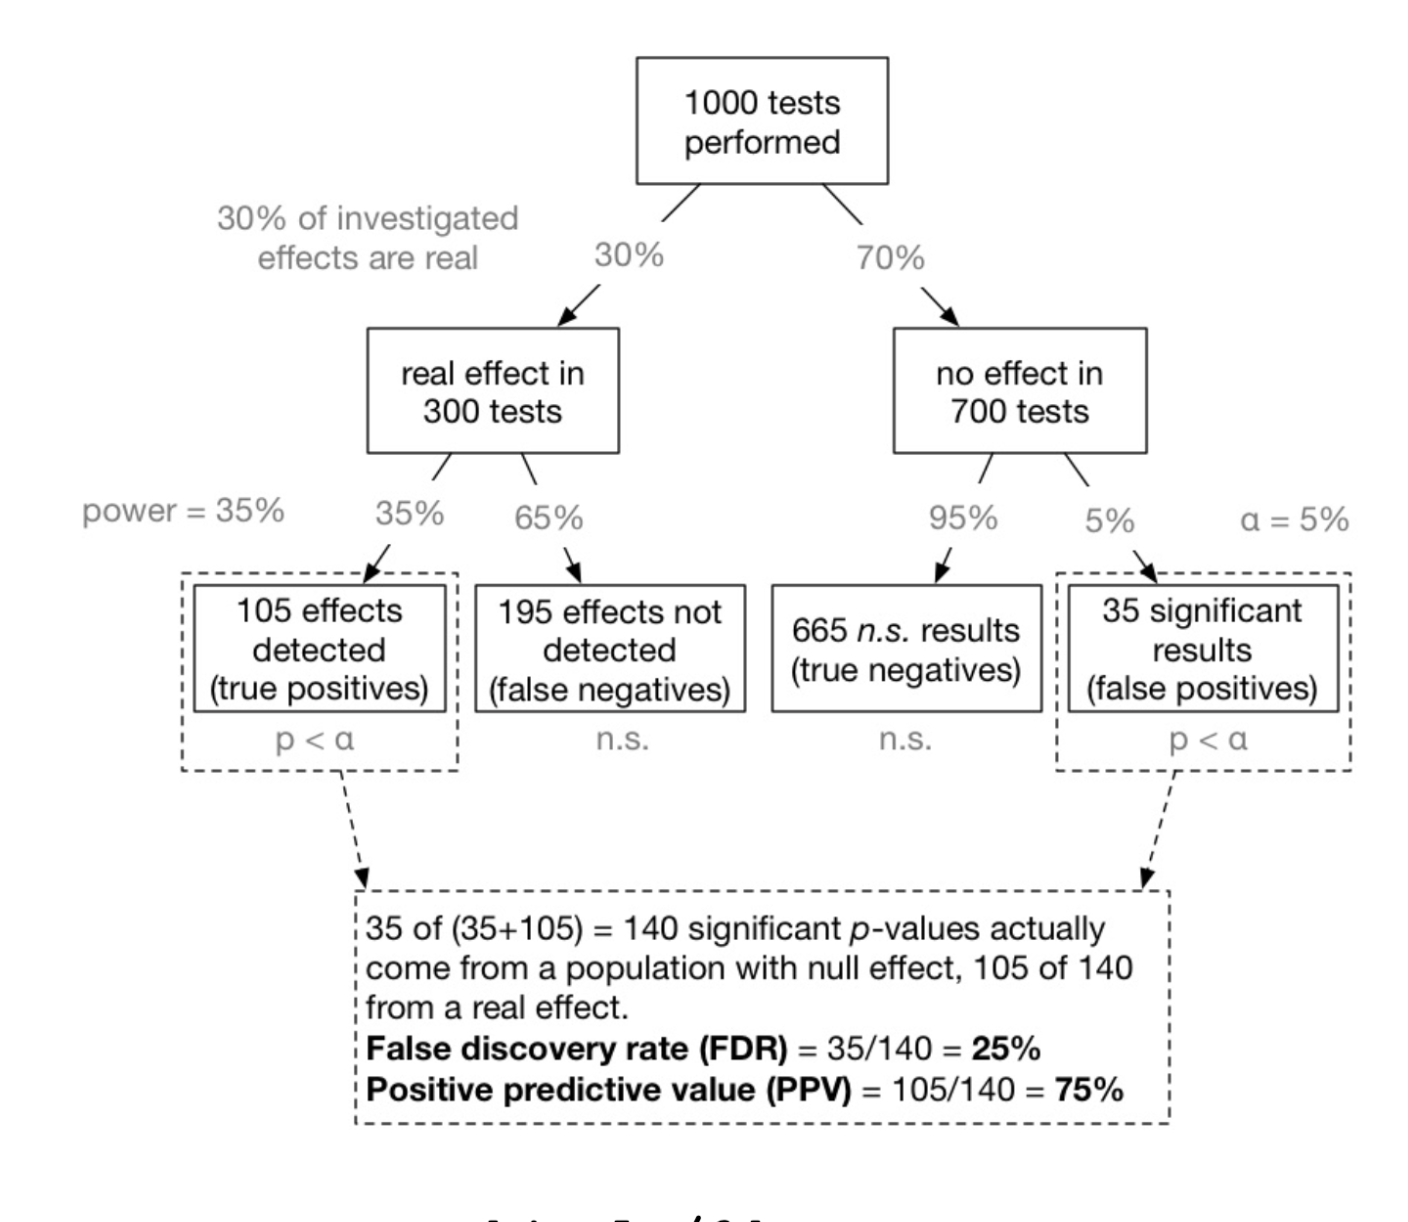
\includegraphics[width=0.5\textwidth]{figures/1.png}
    \caption{
      Answer provided during class.}
    \label{fig:example_figure}
  \end{center}
\end{figure}

\begin{itemize}
  \item Alpha is the false positive rate, and not false discovery rate.
  \item False discovery rate in the quiz above is 35/(35+105)=35 percent.
\end{itemize}

\newpage
\section{Effect Size}

\begin{itemize}
  \item Effect size is anything that might be of interest.
  \item Effect sizes, in this case, are metrics that represent the amount of differences between two sample means. \\
\end{itemize} 


The Cohen's d effect size is very popular in psychology. The following graphs show change in Cohen's d.


\begin{equation}
  d=\frac{M1-M2}{\textit{SD pooled}}
\end{equation}


\begin{figure}[ht]
  \begin{center}
    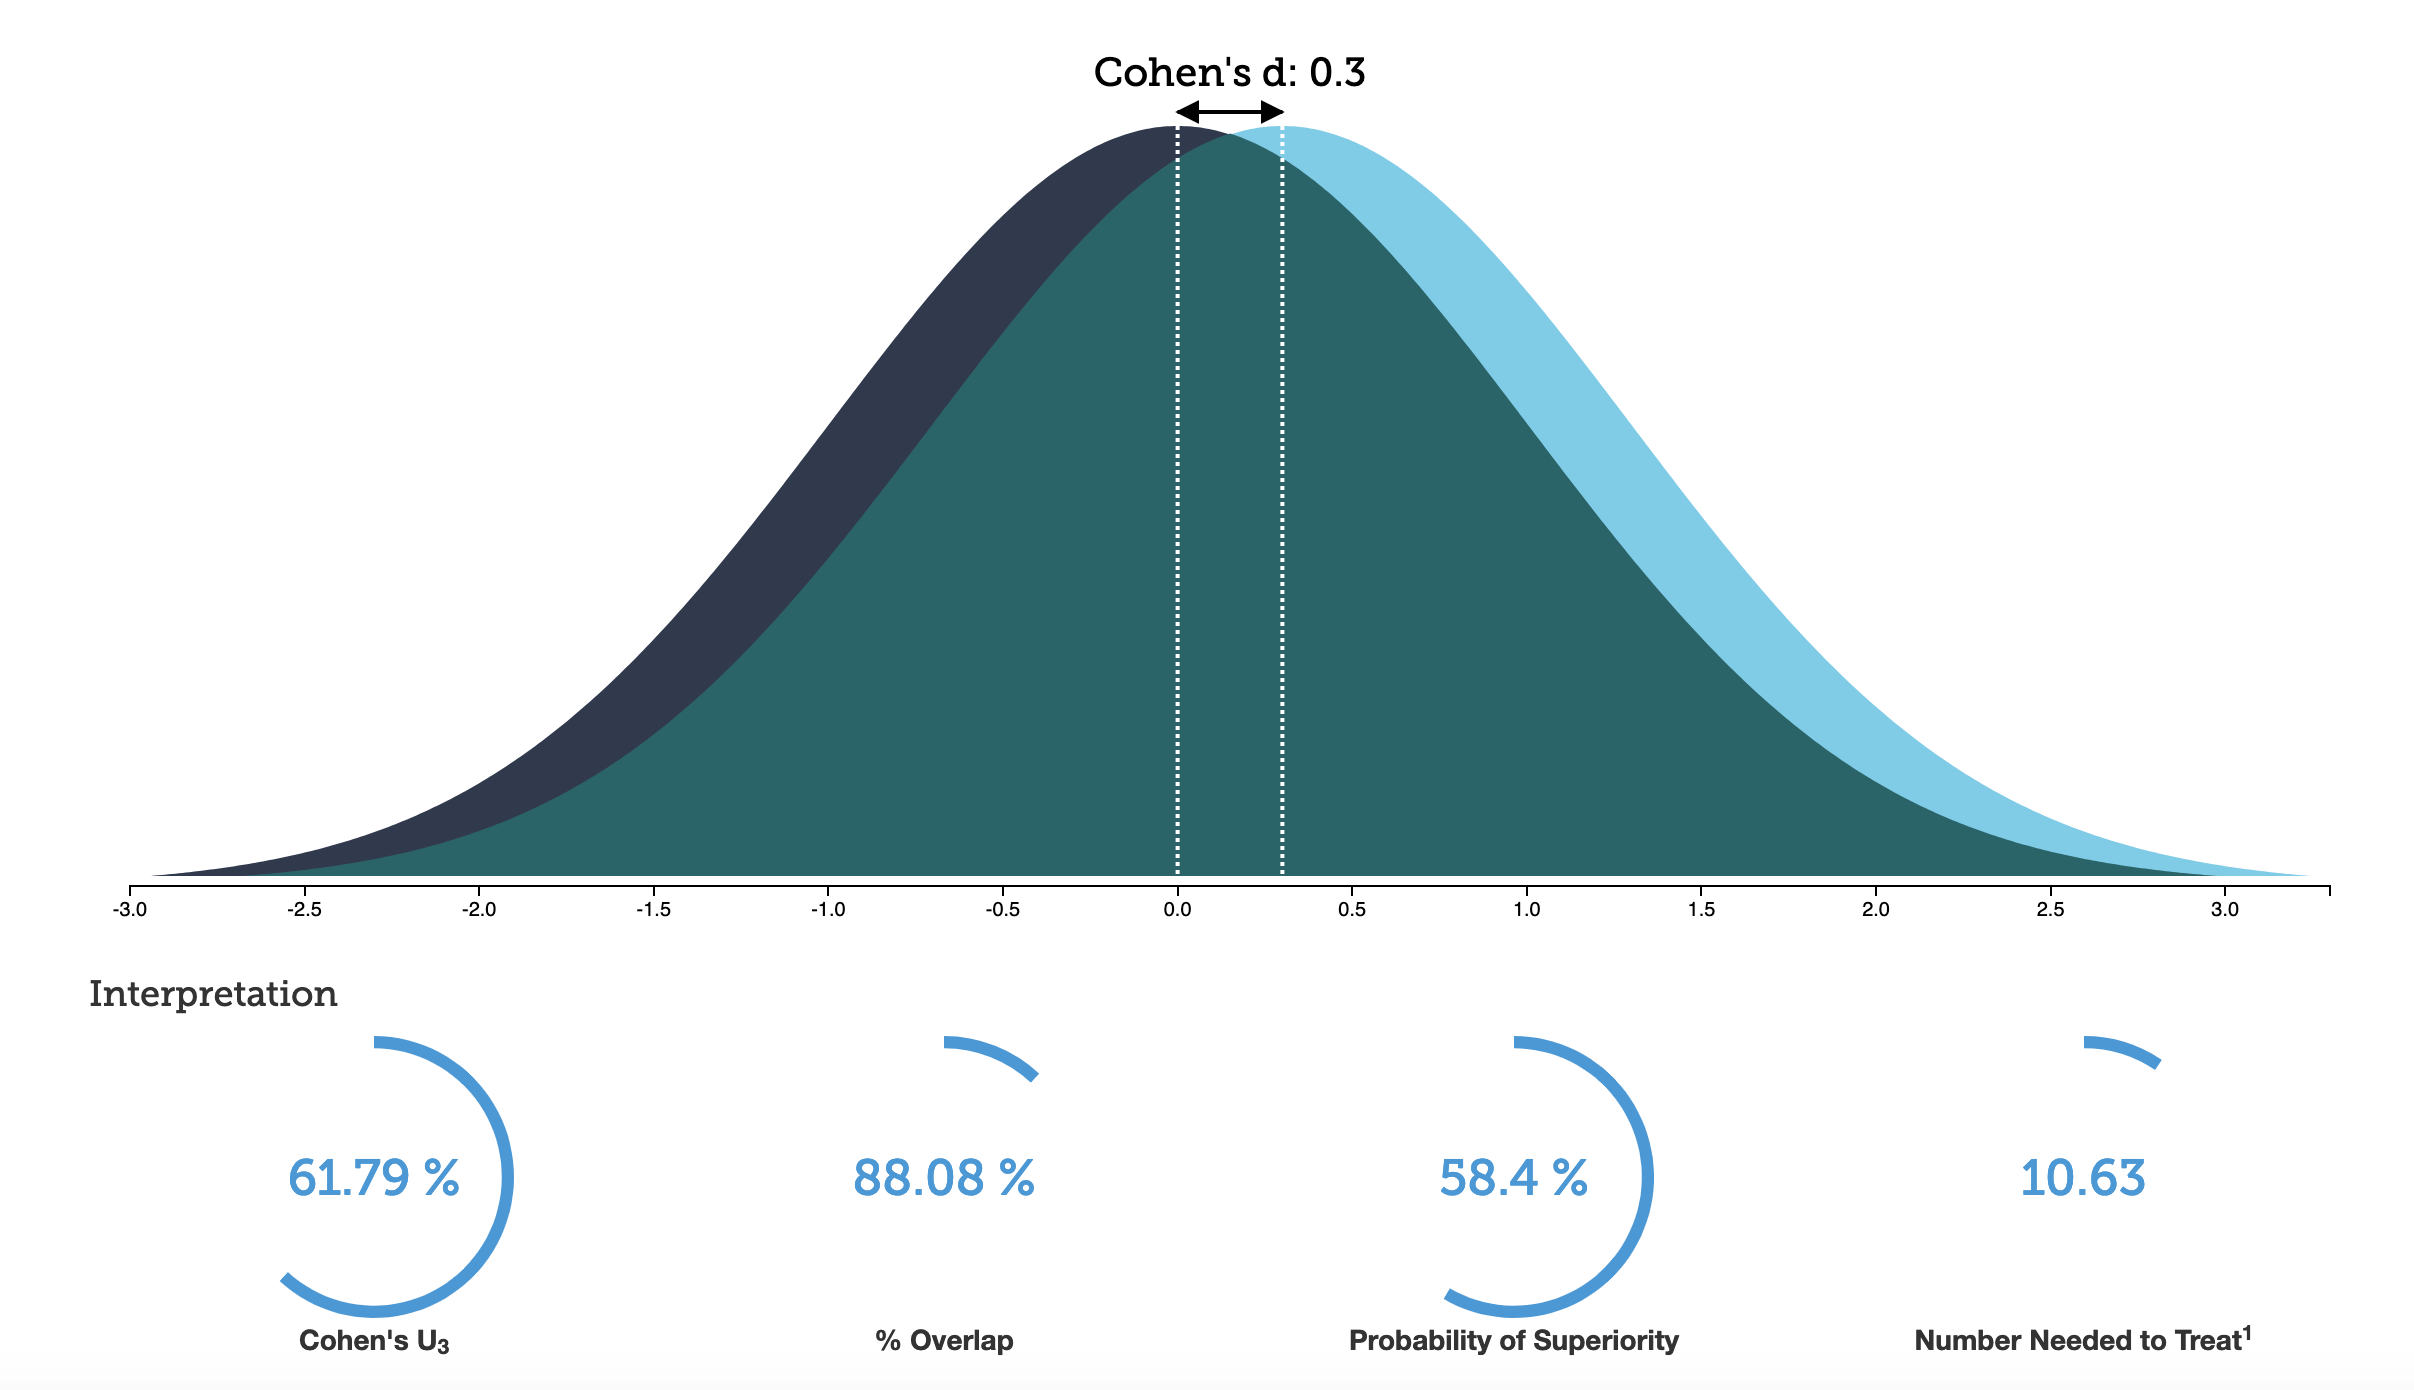
\includegraphics[width=0.6\textwidth]{figures/2.png}
    \caption{
      Cohen's d when it is 0.3.}
    \label{fig:example_figure}
  \end{center}
\end{figure}


\begin{figure}[ht]
  \begin{center}
    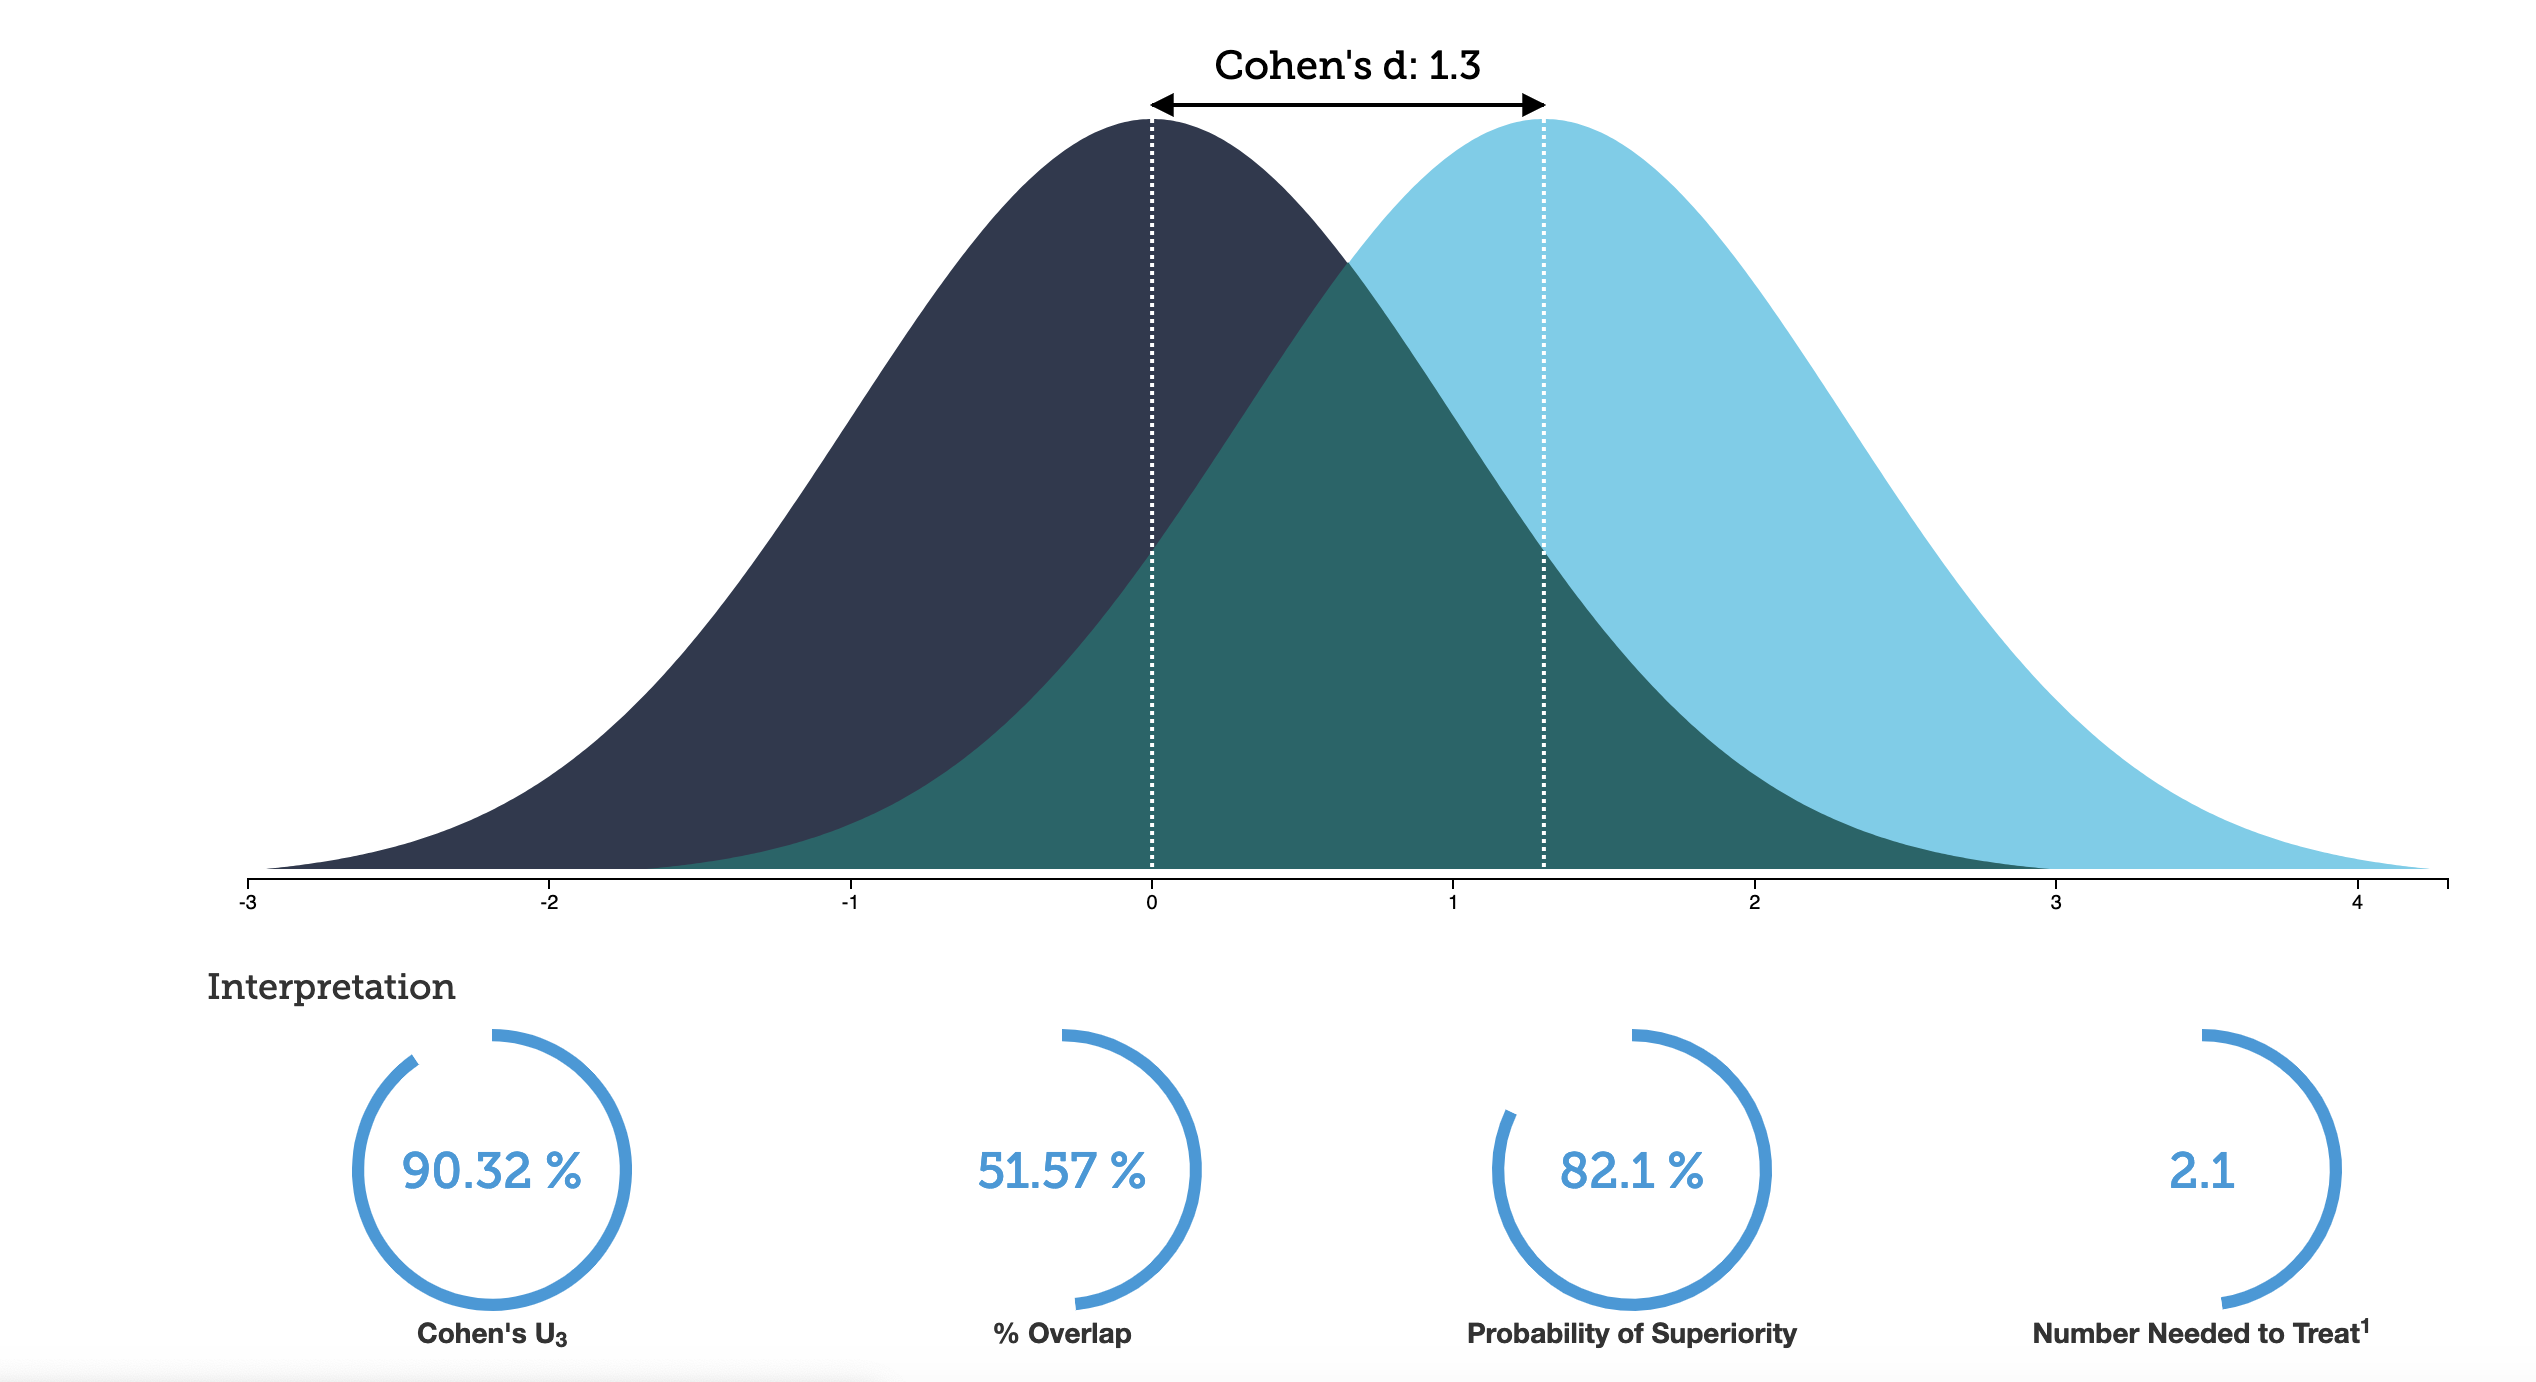
\includegraphics[width=0.6\textwidth]{figures/3.png}
    \caption{
      Cohen's d when it is 1.3.}
    \label{fig:example_figure}
  \end{center}
\end{figure}

Probability of superiority is when probability of treatment is greater than probability of control.\\
When effect size is larger, the probability of superiority increases.\\
Professor's comment: Rejecting the null hypothesis does not tell you difference, the effect size does.\\

\newpage
\section{P-Hacking}

\begin{enumerate}
  \item Study I: musical contrast and subject age
  \item Study II: musical contrast and chronological rejuvenation
\end{enumerate} 

Study I: Reject null hypothesis. Listening to a children's songs does not make people feel older.\\
Study II: Investigated whether listening to old songs makes one really older.\\

Pretty sure listening to adult songs don't make one older. First of all, sample size is small. Songs are different in two studies. One can realize that there are small details that are weird. Actual title of the paper is "False-Positive Psychology: Undisclosed Flexibility in Data Collection and Analysis Allows Presenting Anything as Significant."\\


\begin{figure}[ht]
  \begin{center}
    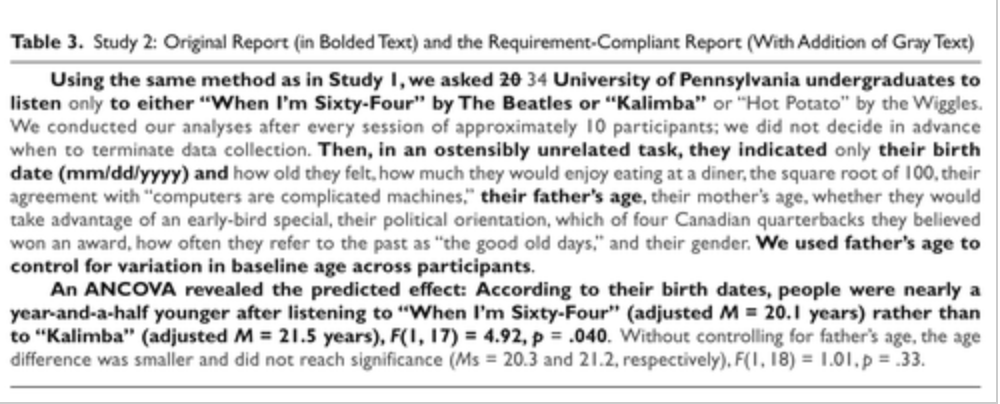
\includegraphics[width=0.6\textwidth]{figures/4.png}
    \caption{
      Paper without overfitting.}
    \label{fig:example_figure}
  \end{center}
\end{figure}


This paper is about manual overfitting, and selective presenting. These types of overfitting can be intentional or not intentional. Exploratory data analysis needs to be dealt very carefully. How do you know you are not fulling yourself? You can check if you are looking for patterns or finding a pattern. You should report everything you did in the paper (disclose all information). One can also pre-register what they are going to do at aspredicted.com. In this article, the authors accomplish two things. First, the authors show that despite empirical psychologists’ nominal endorsement of a low rate of false-positive findings (≤ .05), flexibility in data collection, analysis, and reporting dramatically increases actual false-positive rates. In many cases, a researcher is more likely to falsely find evidence that an effect exists than to correctly find evidence that it does not. The authors  present computer simulations and a pair of actual experiments that demonstrate how unacceptably easy it is to accumulate (and report) statistically significant evidence for a false hypothesis. Second, the authors suggest a simple, low-cost, and straightforwardly effective disclosure-based solution to this problem. The solution involves six concrete requirements for authors and four guidelines for reviewers, all of which impose a minimal burden on the publication process.\\

\end{document}

%%% Local Variables:
%%% mode: latex
%%% TeX-master: t
%%% End:
